\documentclass[a4paper]{article}
\usepackage{hyperref}
\usepackage{graphicx}
\usepackage{caption}
\usepackage{subcaption}
\usepackage{listings}
\usepackage{algorithm}
\usepackage{algpseudocode}
\graphicspath{ {./images/} }

\usepackage{xcolor}

\definecolor{codegreen}{rgb}{0,0.6,0}
\definecolor{codegray}{rgb}{0.5,0.5,0.5}
\definecolor{codepurple}{rgb}{0.58,0,0.82}
\definecolor{backcolour}{rgb}{0.95,0.95,0.92}

\lstdefinestyle{mystyle}{
    backgroundcolor=\color{backcolour},   
    commentstyle=\color{codegreen},
    keywordstyle=\color{magenta},
    numberstyle=\tiny\color{codegray},
    stringstyle=\color{codepurple},
    basicstyle=\ttfamily\footnotesize,
    breakatwhitespace=false,         
    breaklines=true,                 
    captionpos=b,                    
    keepspaces=true, 
    language=Python,               
    numbers=left,                    
    numbersep=5pt,                  
    showspaces=false,                
    showstringspaces=false,
    showtabs=false,                  
    tabsize=2
}

\lstset{style=mystyle}

\title{SON implementation with Spark in Python}
\author{Carli Alberto VR473845\and Fraccaroli Leonardo VR474539}
\date{}

\begin{document}
	\maketitle
	\tableofcontents
	\newpage
	\section{Introduction}
	Finding frequent itemsets is frequently done in data mining domains to understand which items frequently appear together. The definition of ``items'' is beyond the scope of this work. Suffice to say that we treated them as binary variables, listed in a basket only when their value is True. In our project a \textbf{basket} is a list of items that appear together (for example products bought by a customer).
	
	This is an analysis that can be performed on almost any dataset, but is especially suited for domains like e-commerce. It is an interesting challenge to try and take the system to the extreme where the dataset is so large that it does not fit on any single machine's memory and it is more convenient to distribute analysis to multiple compute units.
	
	We tried to imagine ourselves into a big e-commerce company that stores transaction data on a distributed database and wants to periodically analyse data to understand which items are usually bought together. \\
	The data is simply a list of items bought at any time. To store the data in a distributed database we used MongoDB and thus we needed a version of parallel \textbf{Apriori} (an algorithm to find frequent itemsets on a single machine). \\
	We parallelized Apriori by using Spark in Python and using the \textbf{SON} algorithm as proposed in chapter 6.4.4 of the \href{http://www.mmds.org/}{Mining Massive Datasets} book.
	\newpage

	\section{SON}
	In this section we will dissect our implementation of SON through Spark, describing all the steps of computation and their result.
	
	\subsection{SON Algorithm}	
	The algorithm, as described in the book, involves two phases of MapReduce as follows:
	\begin{enumerate}
	\item The mapper basically executes Apriori (or whatever algorithm to find frequent itemsets) on every batch of baskets, extracting all frequent itemsets for each batch. The required frequency (support) is reduced by a factor equal to the number of batches the data is partitioned in, using the following formula:
	\[ batch\_support = basket\_size / total\_data\_size * total\_support \]
	The reducer combines all the frequent itemsets from every batch in a single list. These are \textit{candidate frequent itemsets}.\\
	This step removes false negatives by keeping all the itemsets that are frequent in at least one batch.
	\item The map function takes a batch of the data and counts the occurrence of every candidate itemset.\\
	The reducer adds up the counts from every batch and finally filters out the infrequent ones using the original support.\\
	This step removes false positives by keeping only the itemsets that are globally supported.
	\end{enumerate}
	The result of these phases is the list of \textit{frequent itemsets}.
	
	\subsection{Our Implementation}
	Our implementation expects a $pyspark$ RDD.
	
	\subsubsection{First Map}
	The input data is in the form of a list of lists, where every internal list holds a set of strings, which are the items (fig: \ref{fig:input_data}).
	
	Apriori algorithm is applied to every batch, which returns a list of frequent itemsets (fig: \ref{fig:apriori}). This is done with the $mapPartitions$ function of $pyspark$: 
	\begin{lstlisting}[numbers=none]
.mapPartitions(lambda x: apriori(list(x), support, data_size))
\end{lstlisting}
	where \texttt{x} is a batch, \texttt{support} is the support for the entire dataset and \texttt{data\_size} is the total number of baskets in the entire dataset (they are needed in \texttt{apriori()} to calculate the batch support).
	We will discuss our implementation of Apriori, in details, in section \ref{section:apriori}. We chose not to keep only the largest sets because we saw that there may be cases where the larger set is not globally supported, but the smaller ones are.\\
	Then every itemset is ``emitted'' with a 1, to facilitate the reduce phase:
	\begin{lstlisting}[numbers=none]
.map(lambda x: (x, 1))
\end{lstlisting}
	
	\subsubsection{First Reduce}
	Now the result of the previous step is grouped by key (fig: \ref{fig:grouped}) and the list of counts discarded entirely:
	\begin{lstlisting}
.groupByKey()
.map(lambda x: x[0])
\end{lstlisting}
	The result is the list of all itemsets that appear at least once (fig: \ref{fig:candidate_fi}), which means that they are frequent in at least one batch.\\
	Then the list is collected and broadcasted to all the nodes.
	
	\begin{figure}[h]
		\centering
		
		\begin{subfigure}[b]{0.24\textwidth}
			\centering
			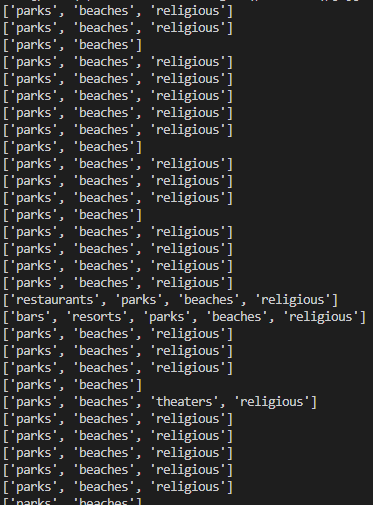
\includegraphics[width=\textwidth]{Baskets.PNG}
         	\caption{Input data}
         	\label{fig:input_data}
		\end{subfigure}
		\hfill
		\begin{subfigure}[b]{0.24\textwidth}
			\centering
			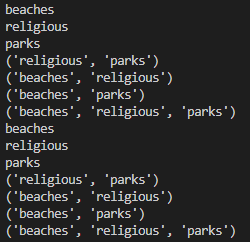
\includegraphics[width=\textwidth]{Batch_fi.PNG}
         	\caption{Apriori on batch}
         	\label{fig:apriori}
		\end{subfigure}
		\hfill
		\begin{subfigure}[b]{0.24\textwidth}
			\centering
			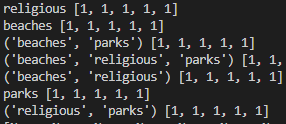
\includegraphics[width=\textwidth]{grouped.PNG}
         	\caption{First reduce}
         	\label{fig:grouped}
		\end{subfigure}
		\hfill
		\begin{subfigure}[b]{0.24\textwidth}
			\centering
			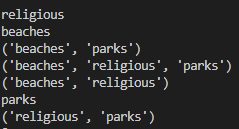
\includegraphics[width=\textwidth]{candidates.PNG}
         	\caption{Candidate frequent itemsets}
         	\label{fig:candidate_fi}
		\end{subfigure}
	\caption{Results of first MapReduce phase}
	\end{figure}
	
	\subsubsection{Second Map}
	Now we need to count the occurrences of every itemset in the whole dataset.\\
	We do it on every partition:
	\begin{lstlisting}[numbers=none]
.mapPartitions(lambda x: count_frequencies(candidate_frequent_itemsets.value, list(x)))
\end{lstlisting}
	The result is a list of tuples where the first element is the itemset and the second is the count for every batch (fig: \ref{fig:counts}).
	
	\subsubsection{Second Reduce}
	Now the itemsets are reduced across partitions by summing counts (fig: \ref{fig:totals}) and then filtered:
	\begin{lstlisting}
.reduceByKey(lambda x, y: x + y)
.filter(lambda x: x[1] / data_size >= support)
\end{lstlisting}	
	The result is the list of every itemset which is supported enough to be considered frequent. Our next step is to filter out all the smaller sets which are included in larger sets.
	
	\begin{figure}[h]
		\centering
		
		\begin{subfigure}[b]{0.4\textwidth}
			\centering
			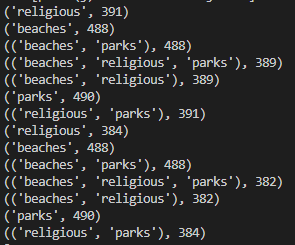
\includegraphics[width=\textwidth]{counts.PNG}
         	\caption{Counts of itemsets for every batch}
         	\label{fig:counts}
		\end{subfigure}
		\hfill
		\begin{subfigure}[b]{0.4\textwidth}
			\centering
			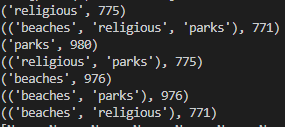
\includegraphics[width=\textwidth]{totals.PNG}
         	\caption{Sum of counts across partitions}
         	\label{fig:totals}
		\end{subfigure}
	\end{figure}
	
	\newpage
	
	\section{Apriori}
	\label{section:apriori}
	
	Apriori is the most used algorithm to find frequent itemsets in a dataset. The algorithm relies on the monotonicity of support by building candidates from smaller sets which are knowingly frequent. This is because it is impossible for an itemset to be frequent if every item it is composed of is frequent by itself. The algorithm \ref{algo:apriori} shows the Apriori pseudocode.
	
	To benchmark SON execution we had to compare it to an implementation of Apriori, which we made ourselves (\textit{Scripts/apriori.py}).
	
\begin{algorithm}
\caption{Apriori pseudocode}
\label{algo:apriori}
\begin{algorithmic}[1]
\Function{apriori}{data, total\_support, total\_db\_size}
	\State $L_1 \gets \{frequent \ 1-itemsets\}$ \Comment{\textcolor{gray}{\emph{\parbox[t]{.3\linewidth}{$L_k$ is the set of truly frequent itemsets of size $k$}}}}
    	\State $k \gets 2$
    	\While{$L_{k-1}$ is not empty}
    		\State create $C_k$ using $L_{k-1}$ (by adding singlets) \Comment{\textcolor{gray}{\emph{\parbox[t]{.3\linewidth}{$C_k$ is the set of candidate itemsets of size $k$}}}}
    		\State count occurrences of each itemset of $C_k$ in $data$
    		\State filter out non-frequent itemsets in $C_k$
    		\State $L_k \gets C_k$
    		\State $k \gets k+1$
    	\EndWhile
\EndFunction
\end{algorithmic}
\end{algorithm}

    In our implementation of the Apriori pseudocode we first extract the items from the data, keep the frequent ones and then use them to build all the candidate couples, count them, filter out infrequent ones and then expand those couples to form triples and so on.
	
	\section{Benchmark}
	We have ran some benchmarks to better understand how SON compares to Apriori.
	
	In order to do so we made a script for the specific purpose of being able to programatically change parameters and 	subsample datasets.
	Also, we implemented a gridsearch to test many parameters. We also added a logging feature to our project to better follow executions and ease debug.
	
	We compared our implementation, both \textbf{based on DB} (using the \href{https://www.mongodb.com/docs/spark-connector/current/}{MongoDB Connector for Spark}, which is kind of a ``real world'' example) and \textbf{in memory} (having all the data locally), to a method $FreqItems$ provided by $pyspark.sql$. 
	This function implements the algorithm proposed by \href{https://doi.org/10.1145/762471.762473}{Karp, Schenker, and Papadimitriou}, which uses a modified version of FP-Tree to be more parallelizeable. This function proved itself to be absurdly fast, at the expense of false positives.
	Both a  `simple' dataset and a `harder' one were used to compare performances.

	\subsection{Datasets}
	The first ``easier'' dataset is from UCI \href{https://archive.ics.uci.edu/ml/datasets/Travel+Reviews#}{(Travel Reviews)} and is composed of averages of scores that every user gave to some
	categories of places on TripAdvisor. We arbitrarily kept only the ones with an average mark above 2.5. This way our dataset is in the form:
	\[ user\_id: category1, category2, \ldots \]
	It is considered ``easy'' because it is very sparse and the number of items is very low (10 items).

	The second ``harder'' dataset is a collection of transactions where some user bought some items in a transaction, again from UCI \href{https://archive.ics.uci.edu/ml/datasets/online+retail}{(Online Retail)}.
	We decided to form transactions on invoices, so we extracted the list of items bought together.
	This way our dataset is in the form:
	\[ invoice\_no: item\_code1, item\_code2, \ldots \]
	It is considered ``harder'' because of the higher number of items (4059).

	\subsection{Database}
	Part of our project was to explore how spark interacts with a database like MongoDB.\\
	We found that exists a \href{https://www.mongodb.com/docs/spark-connector/current/}{MongoDB Connector for Spark} to connect to a MongoDB database and read the data from it as well as 
	write the results back to it.\\
	We had some difficulties because the connector version 10 is not compatible with any spark version and had to check, as well as finding the right place to download the connector from.\\
	Also it is very difficult to work in the environment spark+connector, because the connector is written in scala and spark uses function written in java.\\
	
	The main difference between a local spark instance (e.g. reads from disk and not a database) is that the environment is a $SparkSession$, which allows to use connectors to read and write data from databases as well as repartition it.\\
	A partitioner can be specified to regulate how the data is handled and to change how it is distributed.\\	
	The read data is in the form of a $DataFrame$ which wraps an RDD and allows to use SQL queries on it.\\

	We used this connector to test the difference when the data is stored in a database versus when it is read from disk and found out that there is a appreciable difference in performance, but not as much as we expected.\\

	We tried using spark connected to a sharded database, with a sharded partitioner and while it was easy to use (no particular setup on the spark side) it was really difficult to setup the database with no noticeable execution difference.\\
	So we settled on a single node database with a default partitioner, which in the case of our datasets, always produced a single partition.\\

	\subsection{Results}
	% Setups (CPU, MEMORY, MONGO)
	These tests were performed on an 8 core $i5-8250U @1.6GHz$, with 16 GB DDR4 memory $@2400MHz$, but both the driver and the executor were capped at 4 GB.
	figures \ref{fig:easybenchmark}, \ref{fig:hardbenchmark}

	\begin{figure}[h]
		\centering
		\begin{subfigure}[b]{1\textwidth}
			\centering
			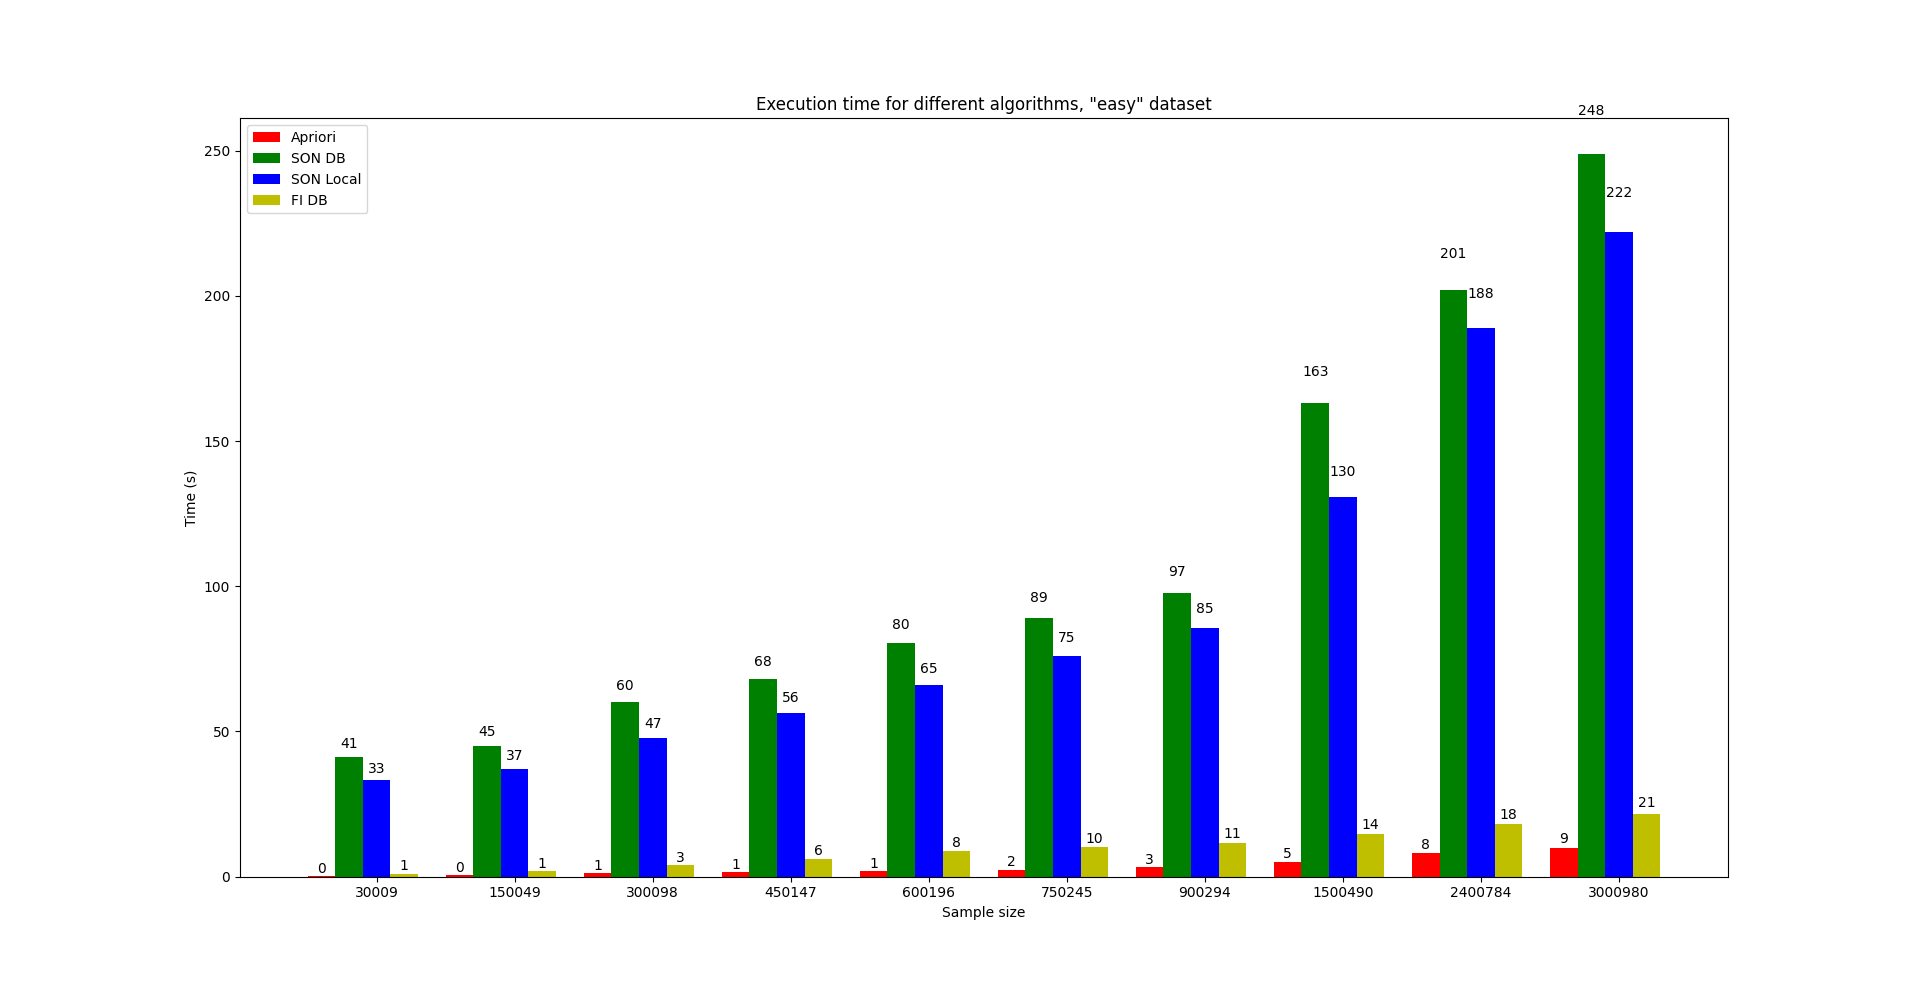
\includegraphics[width=\textwidth]{benchmarkeasy.png}
         	\caption{Easy dataset benchmark results}
         	\label{fig:easybenchmark}
		\end{subfigure}
		\hfill
		
		\begin{subfigure}[b]{1\textwidth}
			\centering
			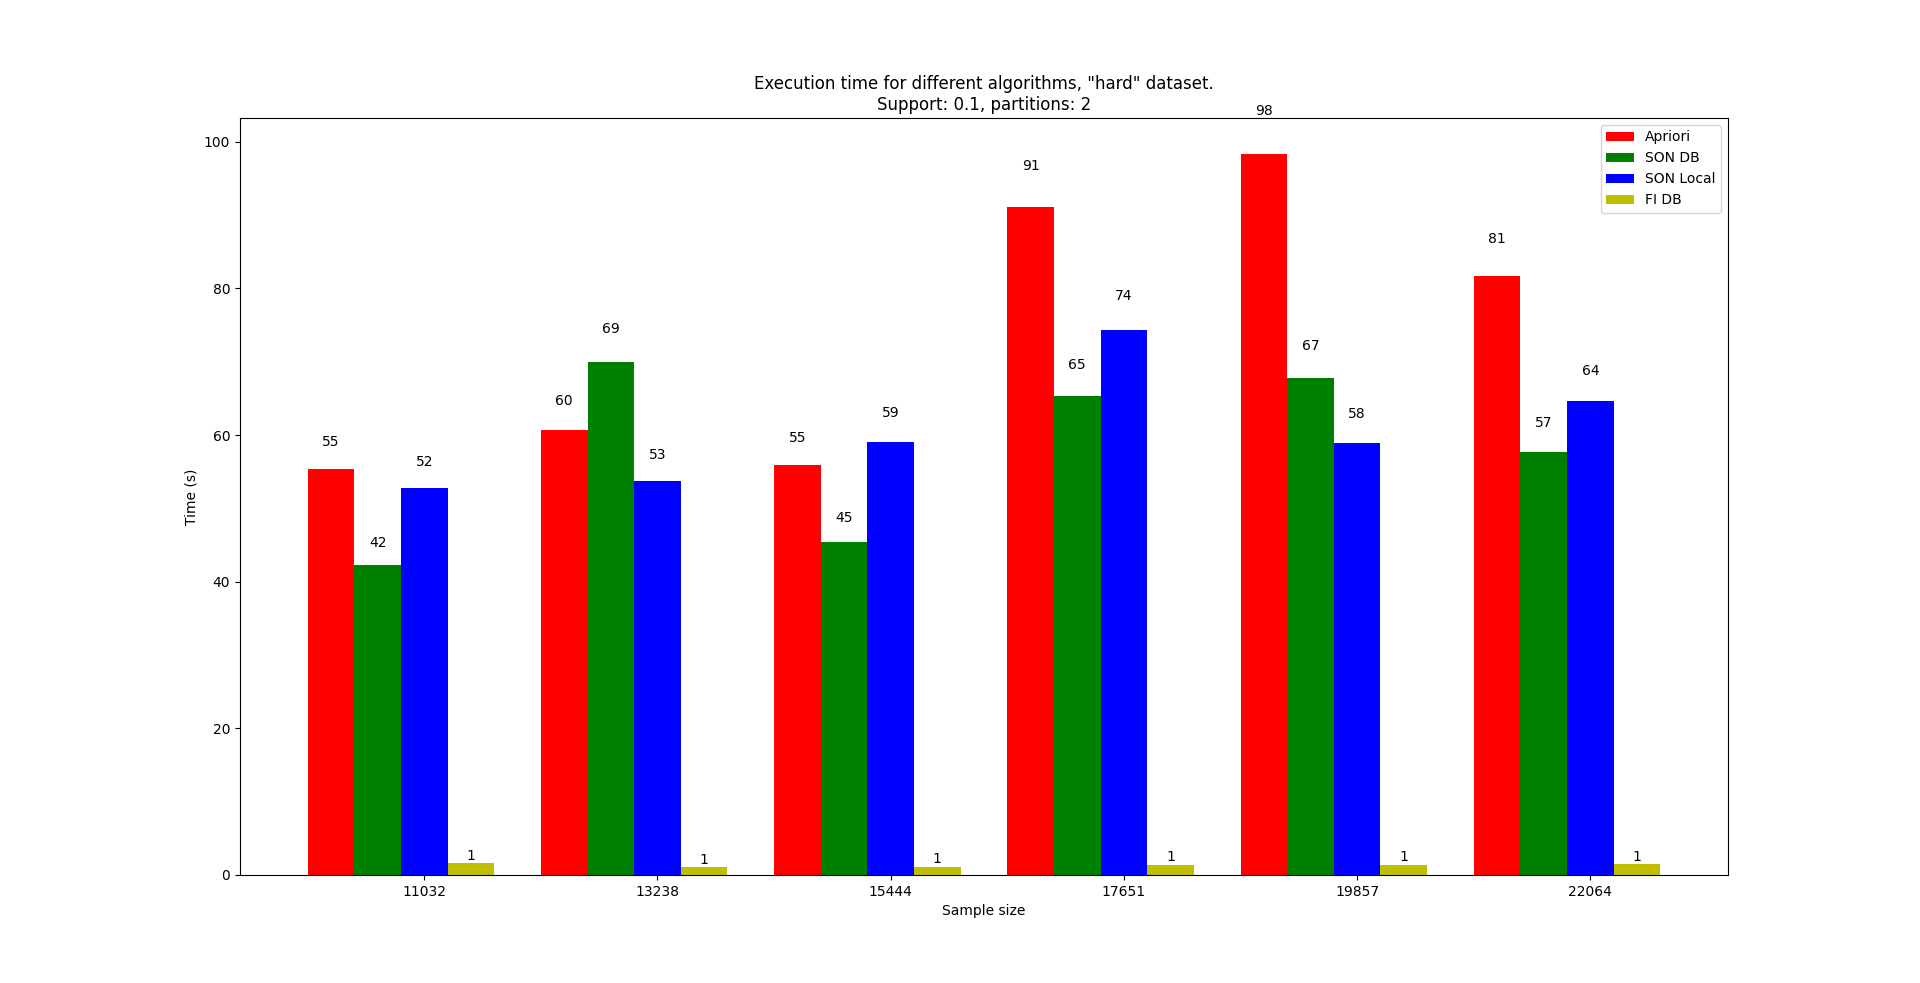
\includegraphics[width=\textwidth]{benchmarkhard.png}
         	\caption{Hard dataset benchmark results}
         	\label{fig:hardbenchmark}
		\end{subfigure}
		\hfill
		
	\end{figure}

	
	\section{Conclusions}
	The main advantage of SON, that we could appreciate in our single machine setup, was the ability to use all the available cores, distributing the load. We also have seen how easy it is connecting pyspark 
	to a distributed database, eventually sharded.
	
	Partitioning in multiple threads seems to not be rewarded both in the local and the database case. We came to the conclusion that the database partitioner optimizes for the database connection, 
	while the local partitioner ($parallelize$ function) optimizes for exploiting all the resources of the machine.\\
	We also found out that a single partition per CPU and not CORE is very efficient.\\
	Furthermore, we have encountered a weird bug where the global support was reduced so much that the support in the partition
	turned out to be less than 1, which caused an explosion in the number of candidates, not because they were actually frequent
	in the partition, but because every item (and their combination in each basket) always appear at least once.\\

	With the testing we have appreciated how SON execution time remains somewhat constant across the dataset sizes, while Apriori execution time grows exponentially with the number of items.
	We could also notice the overhead of the database connection as well as the overhead of spark framework management.
		
\end{document}